\section{Analisi dei requisiti} 
\subsection{Descrizione}
Si vuole realizzare una base di dati che gestisca in maniera efficiente le informazioni relative all’organizzazione del ristorante “La Sofia” a Padova. In particolare si vogliono conoscere i dati relativi a: provviste nel magazzino e nella cantina, contabilità (entrate ed uscite), dipendenti, turni di lavoro e prenotazioni effettuate per il locale. \medskip \\
Di ciascun \textbf{prodotto} si vuole sapere:
\begin{itemize}
    \item Codice idenficativo progessivo numerico
    \item Nome
    \item Quantità presente nel magazzino
    \item Prezzo
    \item Fornitore
\end{itemize}
I prodotti si suddividono in prodotti da frigo, surgelati e prodotti a lunga conservazione oppure bevande. \\
Una bevanda può essere un vino. \\
Ogni vino è caratterizzato da una marca, un'annata e un tipo(rosso fermo, bianco fermo, rosè, frizzante, passito o distillato). \\
Ogni prodotto viene usato per uno o più piatti. \\
Ogni bevanda può essere contenuta in un ordine. \\
Ogni prodotto viene acquistato presso un solo fornitore.\\
Per ogni prodotto, il prezzo deve corrispondere al relativo costo di un'uscita. \\
Per ogni prodotto il nome deve corrispondere ad un ingrediente in almeno un piatto. \\
Per i prodotti da frigo, o freschi, si vuole inoltre conoscere la data di scadenza. \medskip \\
Per quanto riguarda i rifornimenti, per ogni \textbf{fornitore} si vuole sapere:
\begin{itemize}
    \item Codice azienda(Partita IVA) che lo identifica univocamente
    \item Nome azienda
    \item Recapito telefonico
\end{itemize}
Il codice dell'azienda deve corrispondere al fornitore di un vino o di un prodotto. \\
Ogni fornitore vende uno o più prodotti al ristorante, oppure vende uno o più vini per la cantina. \medskip \\
Riguardo alla contabilità, di ogni \textbf{uscita ed entrata} si vuole sapere:
\begin{itemize}
    \item Codice identificativo progessivo numerico
    \item Costo %valore
    \item Data
\end{itemize}
La contabilità comprende sia le entrate che le uscite. \\
Di ogni uscita deve essere specificata anche la motivazione o causale che ha generato il costo. \\
Ogni uscita appartiene ad una spesa effettuata per l'acquisto delle provviste del magazzino. \\
Ogni uscita appartiene ad una spesa effettuata per l'acquisto delle provviste per la cantina. \\
Ogni uscita può costituire un salario dovuto ad un dipendente. \\
Il costo deve corrispondere al prezzo di un prodotto o di un vino. \\
Ogni entrata fa parte dell'incasso derivante da un'ordine. \medskip \\
Di ogni \textbf{Ordine} si vuole sapere:
\begin{itemize}
    \item Numero tavolo 
    \item Piatti
    \item Bevande
    \item Cameriere
    \item Totale
    \item Giorno
    \item Ora
\end{itemize}
Ogni ordine è identificato dal numero del tavolo, il giorno e l'ora. \\
Ogni ordine deve comprendere una bevanda che può essere un vino. \\
Ogni ordine è composto da almeno un piatto.  \\
Ogni ordine è preso e servito da un cameriere. \\
Il cameriere deve avere un codice fiscale corrispondente a quello di un dipendente. \\
Il totale deve corrispondere ad un'entrata. \\
Il nummero del tavolo deve corrispondere ad un tavolo esiste. \medskip \\
Di un \textbf{Piatto} si vuole conoscere:
\begin{itemize}
    \item Codice
    \item Tipo
    \item Ingredienti
\end{itemize}
Il tipo del piatto può essere antipasto, primo, secondo o dessert.\\
Ogni piatto è composto da uno o più ingredienti. \\
Ogni ingrediente deve corrispondere ad un prodotto. \\
Il codice deve corrispondere al piatto di un ordine. \\ 
Ogni piatto può apparire in un ordine. \medskip \\
Per le \textbf{prenotazioni} effettuate per il locale si vuole sapere:
\begin{itemize}
    \item Codice prenotazione che la identifica univocamente
    \item Nome del cliente
    \item Giorno della prenotazione
    \item Ora della prenotazione
    \item Numero di persone al tavolo
\end{itemize}
Il numero di persone per tavolo non può superare il numero di coperti disponibili per quel tavolo. \\ 
Per ogni prenotazione esiste un corrispondente tavolo prenotato. \medskip \\ 
Di ogni \textbf{Tavolo}:
\begin{itemize}
    \item Numero del tavolo che lo identifica univocamente
    \item Quantità di coperti
\end{itemize}
Ad un tavolo può corrispondere una prenotazione. \\
Per ogni tavolo può corrispondere un ordine. \medskip \\
Riguardo al \textbf{personale} invece si vuole sapere:
\begin{itemize}
    \item Codice fiscale, che identifica ogni dipendente univocamente
    \item Nome 
    \item Cognome 
    \item Giorno di riposo
    \item Stipendio
\end{itemize}
Il personale si divide in cuochi, sommelier o camerieri.\\
Lo stipendio deve corrispondere al costo di un'uscita. \\
Il giorno di riposo non può corrispondere ad un giorno nei turni di lavoro. \\
Ogni dipendente non può coprire un turno di lavoro nel suo giorno libero. \medskip \\
Riguardo ai \textbf{turni di lavoro} all’interno del locale, si vuole sapere:
\begin{itemize}
    \item Codice del dipendente
    \item Giorno
    \item Stato, ossia libero o lavorativo
\end{itemize}
Ogni turno di lavoro viene identificato univocamente dal codice del dipendente e il giorno.\\
Un turno non può essere scoperto nella giornata corrente. \\
Il codice del dipendente deve corrispondere al codice fiscale di quest'ultimo. \\
Ogni turno di lavoro comprende l'intera giornata, senza distinzione tra pranzo e cena.\medskip \\

\subsection{Glossario dei termini}
\begin{longtable}{p{2.5cm} p{4.5cm} p{2cm} p{5cm}}
    \toprule
    \textbf{Termine} & \textbf{Descrizione} & \textbf{Sinonimi} & \textbf{Collegamenti}\\ \midrule
    Prodotto & Cibo o bevanda presente nel magazzino & & Fornitore, Contabilità, Piatto, Ordine \\ \midrule
    Fornitore & Azienda fornitrice di prodotti & & Prodotto \\ \midrule
    Contabilità & Uscite ed entrate del ristorante & Spesa & Prodotto, Ordine, Personale \\ \midrule
    Ordine & Ordine effettuato dai clienti & & Contabilità, Piatto, Personale, Tavolo, Prodotto \\ \midrule
    Piatto & Antipasto, primo, secondo o dessert & & Prodotto, Ordine \\ \midrule
    Prenotazione & Prenotazione per un tavolo del ristorante & & Tavolo \\ \midrule
    Tavolo & Tavolo & & Prenotazione, Ordine\\ \midrule
    Personale & Dipendenti a servizio del locale & Dipendente & Contabilità, Ordine, Turni\\ \midrule
    Turni & Turni lavorativi dei dipendenti & & Personale	\\ \midrule
\end{longtable}

\subsection{Operazioni} %almeno 6 query(o/o procedure, viste), 2 trigger, 2 funzioni
\begin{description}
    \item [Operazione 1:]
    \item [Operazione 2:]
    \item [Operazione 3:]
    \item [Operazione 4:]
    \item [Operazione 5:]
    \item [Operazione 6:]
    \item [Operazione 7:]
    \item [Operazione 8:]
\end{description}

\subsection{Strutturazione dei requisiti} 
\begin{longtable}{|p{15.5cm}|}
    \hline
    \textbf{Frasi di carattere generale} \\ \hline
    Si vuole realizzare una base di dati che gestisca in maniera efficiente le informazioni relative all’organizzazione del ristorante “La Sofia” a Padova. In particolare si vogliono conoscere i dati relativi a: provviste nel magazzino e nella cantina, contabilità (entrate ed uscite), dipendenti, turni di lavoro e prenotazioni effettuate per il locale. \\ \hline
\end{longtable}

\begin{longtable}{|p{15.5cm}|}
    \hline
    \textbf{Frasi relative a prodotto} \\ \hline
    Ogni prodotto ha: un codice idenficativo progessivo numerico, un nome, una quantità, un prezzo ed un fornitore.\\
    I prodotti si suddividono in prodotti da frigo, surgelati e prodotti a lunga conservazione
oppure bevande.
Una bevanda può essere un vino.
Ogni vino è caratterizzato da una marca, un’annata e un tipo(rosso fermo, bianco
fermo, rosè, frizzante, passito o distillato).
Ogni prodotto viene usato per uno o più piatti.
Ogni bevanda può essere contenuta in un ordine.
Ogni prodotto viene acquistato presso un solo fornitore.
Per ogni prodotto, il prezzo deve corrispondere al relativo costo di un’uscita.
Per ogni prodotto il nome deve corrispondere ad un ingrediente in almeno un piatto.
Per i prodotti da frigo, o freschi, si vuole inoltre conoscere la data di scadenza.\\ \hline
\end{longtable}

\begin{longtable}{|p{15.5cm}|}
    \hline
    \textbf{Frasi relative a fornitore} \\ \hline
    Ogni fornitore ha: un codice dell'azienda corrispondente alla Partita IVA che lo identifica univocamente, un nome ed un recapito telefonico.\\
    Il codice dell’azienda deve corrispondere al fornitore di un vino o di un prodotto.
Ogni fornitore vende uno o più prodotti al ristorante, oppure vende uno o più vini per la
cantina.
    \\ \hline
\end{longtable}

\begin{longtable}{|p{15.5cm}|}
    \hline
    \textbf{Frasi relative a contabilità} \\ \hline
    Ogni entrata ed uscita ha: un codice idenficativo progressivo numerico, un costo ed una data.
    La contabilità comprende sia le entrate che le uscite.\\
Di ogni uscita deve essere specificata anche la motivazione o causale che ha generato
il costo. 
Ogni uscita appartiene ad una spesa effettuata per l’acquisto delle provviste del magazzino.
Ogni uscita appartiene ad una spesa effettuata per l’acquisto delle provviste per la
cantina.
Ogni uscita può costituire un salario dovuto ad un dipendente.
Il costo deve corrispondere al prezzo di un prodotto o di un vino.
Ogni entrata fa parte dell’incasso derivante da un’ordine.
    \\ \hline
\end{longtable}

\begin{longtable}{|p{15.5cm}|}
    \hline
    \textbf{Frasi relative a ordine} \\ \hline
    Ogni ordine ha: un numero corrispondente al tavolo, i piatti, le bevande, il cameriere che serve al tavolo, un totale, il giorno e l'ora. \\
Ogni ordine è identificato dal numero del tavolo, il giorno e l'ora. 
Ogni ordine deve comprendere una bevanda che può essere un vino. 
Ogni ordine è composto da almeno un piatto.  
Ogni ordine è preso e servito da un cameriere. 
Il cameriere deve avere un codice fiscale corrispondente a quello di un dipendente. 
Il totale deve corrispondere ad un'entrata. 
Il nummero del tavolo deve corrispondere ad un tavolo esiste.
    \\ \hline
\end{longtable}

\begin{longtable}{|p{15.5cm}|}
    \hline
    \textbf{Frasi relative a piatto} \\ \hline
    Un piatto ha: un codice,un tipo, una serie di ingredienti.
Il tipo del piatto può essere antipasto, primo, secondo o dessert.
Ogni piatto è composto da uno o più ingredienti. 
Ogni ingrediente deve corrispondere ad un prodotto. 
Il codice deve corrispondere al piatto di un ordine. 
Ogni piatto può apparire in un ordine.
    \\ \hline
\end{longtable}

\begin{longtable}{|p{15.5cm}|}
    \hline
    \textbf{Frasi relative a prenotazione} \\ \hline
    Ogni prenotazione ha: un codice prenotazione che la identifica univocamente, un nome del cliente prenotante, il giorno della prenotazione, l'ora della prenotazione, un numero di persone al tavolo. 
Il numero di persone per tavolo non può superare il numero di coperti disponibili per quel tavolo. 
Per ogni prenotazione esiste un corrispondente tavolo prenotato.
    \\ \hline
\end{longtable}

\begin{longtable}{|p{15.5cm}|}
    \hline
    \textbf{Frasi relative a tavolo} \\ \hline
    Ogni tavolo ha: un numero del tavolo che lo identifica univocamente, una quantità di coperti. \\
Ad un tavolo può corrispondere una prenotazione. 
Per ogni tavolo può corrispondere un ordine.
    \\ \hline
\end{longtable}

\begin{longtable}{|p{15.5cm}|}
    \hline
    \textbf{Frasi relative a personale} \\ \hline
    Ogni dipendente ha: un codice fiscale, che identifica ogni dipendente univocamente, un nome ed un cognome, il giorno di riposo, uno stipendio. \\
    Il personale si divide in cuochi, sommelier o camerieri.
    Lo stipendio deve corrispondere al costo di un'uscita. 
    Il giorno di riposo non può corrispondere ad un giorno nei turni di lavoro. 
    Ogni dipendente non può coprire un turno di lavoro nel suo giorno libero.
    \\ \hline
\end{longtable}

\begin{longtable}{|p{15.5cm}|}
    \hline
    \textbf{Frasi relative a turni di lavoro} \\ \hline
    Ogni turno di lavoro ha: un codice del dipendente, un giorno ed uno statoche può essere libero o lavorativo. \\
Ogni turno di lavoro viene identificato univocamente dal codice del dipendente e il giorno.
Un turno non può essere scoperto nella giornata corrente. 
Il codice del dipendente deve corrispondere al codice fiscale di quest'ultimo. 
Ogni turno di lavoro comprende l'intera giornata, senza distinzione tra pranzo e cena.
    \\ \hline
\end{longtable}

%\begin{longtable}{|p{15.5cm}|}
    %\hline
    %\textbf{Frasi relative a } \\ \hline
    %\\ \hline
%\end{longtable}

\section{Schema concettuale} %Schema ER
%Immagine
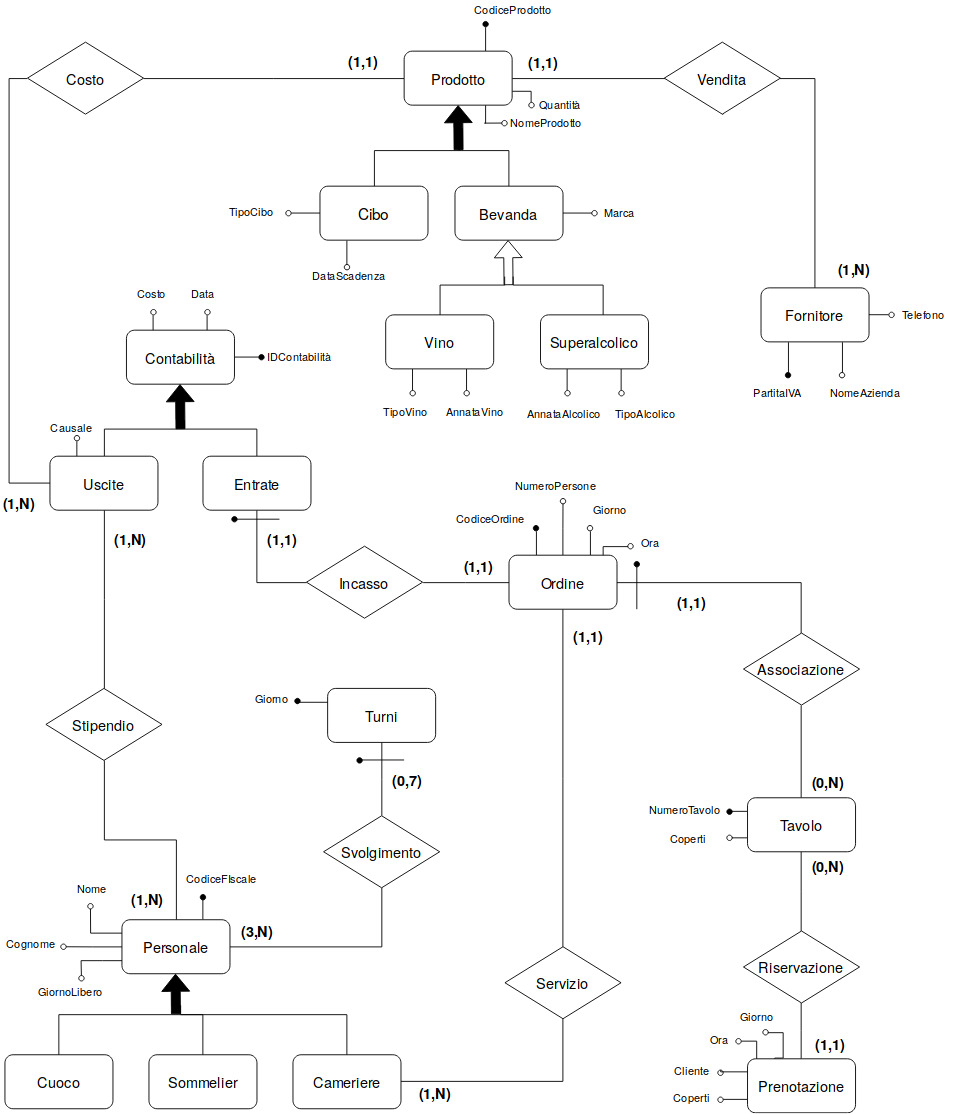
\includegraphics[width=1.1\textwidth]{doc/schema}
%Eventuali note

\subsection{Dizionario dei dati}
\textbf{Lista delle entità}
\begin{longtable}{p{2.5cm} p{4cm} p{5cm} p{2.5cm}}
    \toprule
    \textbf{Enità} & \textbf{Descrizione} &   \textbf{Attributi} & \textbf{Identificatore}\\ \midrule
    Prodotto & Cibo o bevanda presente nel magazzino & Codice, Nome, Quantità, Prezzo, Fornitore&Codice\\ \midrule
    Prodotto a lunga conservazione  &Prodotto con scadenza a lungo termine &Eredita da prodotto &Codice\\ \midrule
    Prodotto fresco	&prodotto da frigo&Eredita da prodotto, Data di scadenza&Codice\\ \midrule
    Prodotto surgelato&Prodotto conservato in congelatore&Eredita da prodotto	&Codice\\ \midrule
    Bevanda	&Bevanda analcolica, birra o vino&Eredita da prodotto&Codice\\ \midrule
    Vino&Bevanda alcolica&Eredita da bevanda, Annata, Marca, Tipo&Codice\\ \midrule
    Fornitore &Azienda fornitrice di prodotti&Partita iva, Nome azienda, Recapito telefonico&Partita iva\\ \midrule
    Contabilità&insieme di entrate ed uscite di denaro&Codice, Costo, Data &Codice\\ \midrule
    Entrata&guadagno del ristorante	&Eredita da contabilità&Codice\\ \midrule
    Uscita&spese del ristorante&Eredita da contabilità, Causale	&Codice\\ \midrule
    Ordine&Ordine effettuato da un cliente	&Numero tavolo, Piatti, Bevande, Cameriere, Totale, Giorno, Ora&Numero tavolo, Giorno, Ora\\ \midrule
    Piatto&Antipasto, primo, secondo o dessert&Codice, Tipo, Ingredienti&Codice\\ \midrule
    Prenotazione&Prenotazione per un tavolo del ristorante&Codice, Nome cliente, Giorno, Ora, Numero di persone&Codice\\ \midrule
    Tavolo&Tavolo&Numero, Coperti&Numero\\ \midrule
    Personale &Dipendenti a servizio del locale	&Codice fiscale, Nome, Cognome, Giorno libero, Stipendio&Codice Fiscale\\ \midrule
    Cuoco&Dipendente in cucina&Eredita da personale&Codice Fiscale\\ \midrule
    Sommelier&Dipendente addetto ai vini &Eredita da personale&Codice Fiscale\\ \midrule
    Cameriere&Dipendente che serve ai tavoli&Eredita da personale&Codice Fiscale\\ \midrule
    Turno &Turno lavorativo di un dipendente&Giorno, Stato, Dipendente&Giorno\\ 
    \bottomrule	
\end{longtable}

%Lista delle generalizzazioni

\begin{comment}
    \textbf{Lista delle relazioni} %Dalla relazione di La casa del pellegrino
\begin{longtable}{p{2.5cm} p{3cm} p{5.5cm} p{3cm}}
    \midrule
    \textbf{Relazione} & \textbf{Descrizione} & \textbf{Cardinalità} & \textbf{Entità coinvolte} \\ \midrule
    Vendita & Associa il prodotto al suo fornitore & Un prodotto è venduto da un solo fornitore (1,1) \newline Un fornitore vende uno o più prodotti (1,N) & Prodotto, Fornitore \\ \midrule
    Creazione & Associa il prodotto al piatto & Un prodotto crea uno o più piatti (1,N) \newline Un piatto è creato da almeno un prodotto (1,N) & Prodotto, Piatto \\ \midrule
    Costo & Associa il prezzo del prodotto all'uscita di denaro & Un prodotto costituisce una o più uscite (1,N) \newline Un uscita è costituita da uno o più prodotti (1,N) & Prodotto, Uscite \\ \midrule
    Appartenenza & Associa la bevanda all'ordine & Una bevanda può appartenere ad uno o più ordini (0,N) \newline Un ordine contiene almeno una bevanda (1,N) & Bevanda, Ordine \\ \midrule
    Composizione & Associa il piatto all'ordine & Un piatto può comporre uno o più ordini (0,N) \newline Un ordine è composto da almeno un piatto (1,N) & Piatto, Ordine \\ \midrule
    Incasso & Associa l'ordine all'entrata di denaro & Un ordine genera una sola entrata (1,1) \newline Un'entrata è generata da un solo ordine (1,1) & Ordine, Entrate \\ \midrule
    Associazione & Associa l'ordine al tavolo & Un ordine è associato ad un solo tavolo (1,1) \newline Un tavolo può essere associato ad uno o più ordini (0,N) & Ordine, Tavolo \\ \midrule
    Riservazione & Associa il tavolo alla prenotazione & Un tavolo può essere riservato da uno o più clienti (0,N) \newline Una prenotazione riserva un solo tavolo (1,1) & Tavolo, Prenotazione \\ \midrule
    Servizio & Associa l'ordine al cameriere & Un ordine viene servito da un solo cameriere (1,1) \newline Un cameriere serve uno o più ordini (1,N) & Ordine, Cameriere \\ \midrule
    Svolgimento & Associa il dipendente al turno di lavoro & Un dipendente può svolgere un turno (0,7) \newline Un turno è svolto da almeno un dipendente di ciascuna categoria (3,N) & Personale, Turni \\ \midrule
    Stipendio & Associa lo stipendio del dipendente all'uscita di denaro & Un dipendente genera un'uscita mensile (1,N) \newline Un' uscita è costituita da uno o più stipendi (1,N) & Personale, Uscite \\ \bottomrule
\end{longtable}
\end{comment}


\textbf{Lista delle relazioni} %Come nel libro
\begin{longtable}{p{2.5cm} p{5.5cm} p{3.5cm} p{2.5cm}}
    \midrule
    \textbf{Relazione} & \textbf{Descrizione} & \textbf{Cardinalità} & \textbf{Attributi} \\ \midrule
    Vendita & Associa il prodotto al suo fornitore & Prodotto(1,1) \newline Fornitore(1,N) &  \\ \midrule
    Creazione & Associa il prodotto al piatto & Prodotto(1,N) \newline Piatto(1,N) & \\ \midrule
    Costo & Associa il prezzo del prodotto all'uscita di denaro & Prodotto(1,N) \newline Uscita(1,N) & \\ \midrule
    Appartenenza & Associa la bevanda all'ordine & Bevanda(0,N) \newline Ordine(1,N) &  \\ \midrule
    Composizione & Associa il piatto all'ordine & Piatto(0,N) \newline Ordine(1,N) &  \\ \midrule
    Incasso & Associa l'ordine all'entrata di denaro & Ordine(1,1) \newline Entrata(1,1) &  \\ \midrule
    Associazione & Associa l'ordine al tavolo & Ordine(1,1) \newline Tavolo(0,N) &  \\ \midrule
    Riservazione & Associa il tavolo alla prenotazione & Tavolo(0,N) \newline Prenotazione(1,1) &  \\ \midrule
    Servizio & Associa l'ordine al cameriere & Ordine(1,1) \newline Cameriere(1,N) & \\ \midrule
    Svolgimento & Associa il dipendente al turno di lavoro & Dipendente(0,7) \newline Turno(3,N) & \\ \midrule
    Stipendio & Associa lo stipendio del dipendente all'uscita di denaro & Dipendente(1,N) \newline Uscita(1,N) &  \\ \bottomrule
\end{longtable}

%Lista delle regole aziendali / regole di vincolo
